\documentclass[]{beamer}
\usepackage[utf8]{inputenc}
\usepackage[english]{babel}
\usepackage{url}
\usepackage{hyperref}
\hypersetup{pdfsubject={Slides of the lightning talk about Fail2Ban
    given at PyCon 2014},%
  pdftitle={Fail2Ban -- keep your boxes skiddie-free},%
  pdfauthor={Yaroslav O. Halchenko},
  pdfkeywords={Fail2Ban, security},%
  colorlinks,citecolor=blue,linkcolor=green,urlcolor=blue}

% reuse the style but we need
\input{../sty/beamer-debian.tex}
\setbeamertemplate{blocks}[default]

\let\Tiny\tiny% http://tex.stackexchange.com/q/58087/5764
\usepackage{fancyvrb}% http://ctan.org/pkg/fancyvrb

\input{s-common}

\title[Fail2Ban]{Fail2Ban -- keep your boxes skiddie-free}
% PyMVPA and NeuroDebian}
\author[yoh AKA Yarik]{Yaroslav O. Halchenko
  \href{mailto: yoh@debian.org}{yoh@debian.org}}
\institute[Dartmouth, (Neuro)Debian]{\href{http://www.dartmouth.edu}{Dartmouth College},
\href{http://www.debian.org}{Debian Project}
%\href{http://neuro.debian.net}{NeuroDebian},
%\href{http://www.pymvpa.org}{PyMVPA}
}
\date[PyCon 2014]{PyCon 2014, Montreal, Canada}

\urlstyle{same}

%%%%%%%%%%%%%%%%%%%%%%%%%%%%%%%%%%%%%%%%%%%%%%%%%%%%%%%%

\begin{document}

{%\PYMVPABIG
 % TODO: create NDBG image
 \NDPYMVPABG
 %\SWIRLBG
 %\NDBG
 \frame{\titlepage}}

\begin{frame}{}
\begin{center}
\includegraphics[width=0.6\textwidth]{pics/logo.pdf}
\\
\href{http://fail2ban.org}{fail2ban.org}
\end{center}
\end{frame}

\begin{frame}{}
\begin{center}
\Large Who cares?
\end{center}
\end{frame}

\begin{frame}{Who cares?}
\begin{center}
\only<1>{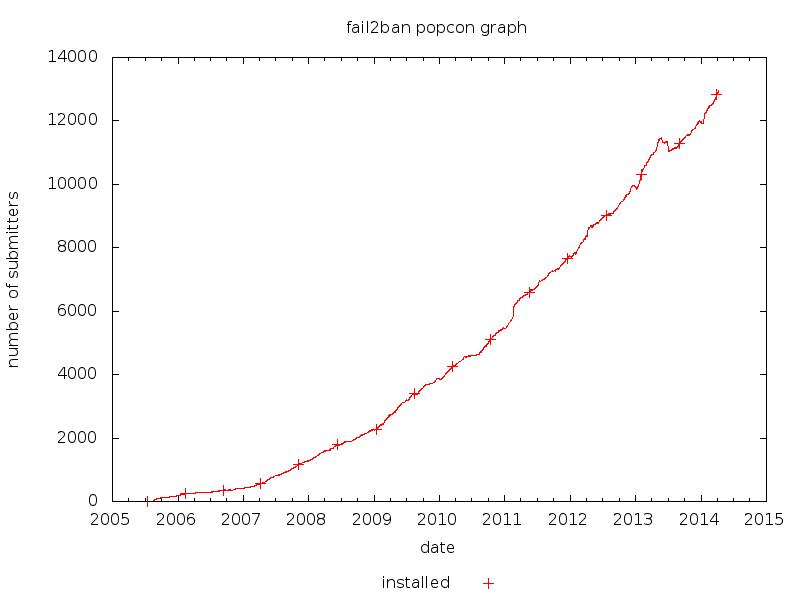
\includegraphics[width=\textwidth]{popcon-abs.png}}
\only<2>{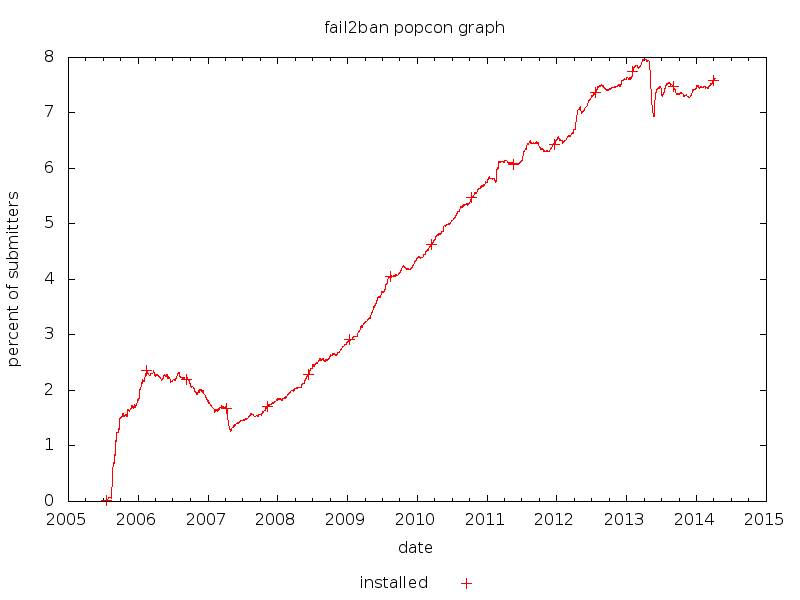
\includegraphics[width=\textwidth]{popcon-rel.png}}
\end{center}
\end{frame}



\begin{frame}[t,fragile]{What is it for?}
\begin{Verbatim}[commandchars=\\\{\},fontsize=\scriptsize]
> tail -f /var/log/auth.log | grep sshd
Jun 2 16:47:48 i sshd[1]: Failed password for X from 1.2.3.4 port 59926
Jun 2 16:47:48 i sshd[1]: Failed password for X from 1.2.3.4 port 59926
Jun 2 16:47:48 i sshd[1]: Failed password for X from 1.2.3.4 port 59926
Jun 2 16:47:48 i sshd[1]: Failed password for X from 1.2.3.4 port 59926
Jun 2 16:47:48 i sshd[1]: Failed password for X from 1.2.3.4 port 59926
Jun 2 16:47:49 i sshd[1]: Failed password for X from 1.2.3.4 port 59926
Jun 2 16:47:49 i sshd[1]: Failed password for X from 1.2.3.4 port 59926
Jun 2 16:47:49 i sshd[1]: Failed password for X from 1.2.3.4 port 59926
Jun 2 16:47:49 i sshd[1]: Failed password for X from 1.2.3.4 port 59926
Jun 2 16:47:49 i sshd[1]: Failed password for X from 1.2.3.4 port 59926
Jun 2 16:47:49 i sshd[1]: Failed password for X from 1.2.3.4 port 59926
Jun 2 16:47:49 i sshd[1]: Failed password for X from 1.2.3.4 port 59926
Jun 2 16:47:49 i sshd[1]: Failed password for X from 1.2.3.4 port 59926
Jun 2 16:47:49 i sshd[1]: Failed password for X from 1.2.3.4 port 59926
\end{Verbatim}

\end{frame}


\begin{frame}[t,fragile]{What is it for?}
\begin{Verbatim}[commandchars=\\\{\},fontsize=\scriptsize]
> tail -f /var/log/auth.log | grep sshd
Jun 2 16:47:48 i sshd[1]: Failed password for X from 1.2.3.4 port 59926
Jun 2 16:47:48 i sshd[1]: Failed password for X from 1.2.3.4 port 59926
Jun 2 16:47:48 i sshd[1]: Failed password for X from 1.2.3.4 port 59926
Jun 2 16:47:48 i sshd[1]: Failed password for X from 1.2.3.4 port 59926
Jun 2 16:47:48 i sshd[1]: Failed password for X from 1.2.3.4 port 59926
Jun 2 16:47:49 i sshd[1]: Failed password for X from 1.2.3.4 port 59926
Jun 2 16:47:49 i sshd[1]: Failed password for X from 1.2.3.4 port 59926
Jun 2 16:47:49 i sshd[1]: Failed password for X from 1.2.3.4 port 59926
Jun 2 16:47:49 i sshd[1]: Failed password for X from 1.2.3.4 port 59926
Jun 2 16:47:49 i sshd[1]: Failed password for X from 1.2.3.4 port 59926
Jun 2 16:47:49 i sshd[1]: Failed password for X from 1.2.3.4 port 59926
Jun 2 16:47:49 i sshd[1]: Failed password for X from 1.2.3.4 port 59926
Jun 2 16:47:49 i sshd[1]: Failed password for X from 1.2.3.4 port 59926
Jun 2 16:47:49 i sshd[1]: Failed password for X from 1.2.3.4 port 59926
\end{Verbatim}

%\only<2>{
%\alert
\begin{Verbatim}[commandchars=\\\{\},fontsize=\scriptsize]
...
\alert{Jun 3 02:00:00 i sshd[1]: Accepted password for X from 1.2.3.4 port 59926}
\end{Verbatim}
%}
%}
\end{frame}

\begin{frame}[fragile]{After ``apt-get install fail2ban logwatch''}

\begin{Verbatim}[commandchars=\\\{\},fontsize=\scriptsize]
> tail -f /var/log/auth.log | grep sshd
Jun 2 16:47:48 i sshd[1]: Failed password for joe from 1.2.3.4 port 59926 ssh2
Jun 2 16:47:48 i sshd[1]: Failed password for joe from 1.2.3.4 port 59926 ssh2
Jun 2 16:47:48 i sshd[1]: Failed password for joe from 1.2.3.4 port 59926 ssh2

> tail -f /var/log/fail2ban.log
2013-06-02 06:47:14 fail2ban.actions[4]: WARNING [apache] Ban 1.2.3.4
2013-06-02 06:57:15 fail2ban.actions[4]: WARNING [apache] Unban 1.2.3.4
\end{Verbatim}

\begin{block}{Next day logwatch email}

\begin{Verbatim}[commandchars=\\\{\},fontsize=\scriptsize]
 --------------------- fail2ban-messages Begin ------------------------

 Banned services with Fail2Ban:                          Bans:Unbans
    ssh:                                                    [  3:3  ]

 ---------------------- fail2ban-messages End -------------------------
\end{Verbatim}
\end{block}

\end{frame}

\begin{frame}{}
\begin{center}
\Large How does \emph{it} know?
\end{center}
\end{frame}

\begin{frame}[fragile]{1. Filter}

\begin{block}{/etc/fail2ban/filters.d/sshd.conf}
{\scriptsize
\begin{verbatim}
[INCLUDES]
before = common.conf

[Definition]
_daemon = sshd

failregex = ^%(__prefix_line)s(?:error: PAM: )?[aA]uthentication
             (?:failure|error) for .* from <HOST>( via \S+)?\s*$
            ^%(__prefix_line)s(?:error: PAM: )?User not known to
             the underlying authentication module for .* from <HOST>\s*$
            ...
\end{verbatim}
}
\end{block}
\end{frame}


\begin{frame}[fragile]{2. Action}

\begin{block}{/etc/fail2ban/action.d/iptables.conf}
{\scriptsize
\begin{verbatim}
[Definition]
actionstart=iptables -N f2b-<name>
            iptables -A f2b-<name> -j RETURN
            iptables -I <chain> -p <protocol> --dport <port> -j f2b-<name>

actionstop=iptables -D <chain> -p <protocol> --dport <port> -j f2b-<name>
           iptables -F f2b-<name>
           iptables -X f2b-<name>

actioncheck=iptables -n -L <chain> | grep -q 'f2b-<name>[ \t]'

actionban=iptables -I f2b-<name> 1 -s <ip> -j <blocktype>

actionunban=iptables -D f2b-<name> -s <ip> -j <blocktype>
\end{verbatim}
}
\end{block}
\end{frame}


\begin{frame}[fragile]{3. Jail (= Filter + Action(s))}

\begin{block}{/etc/fail2ban/jail.conf}
{\scriptsize
\begin{verbatim}
[DEFAULT]

bantime = 600

[sshd]

enabled  = true
filter   = sshd
action   = iptables[name=SSH, port=ssh, protocol=tcp]
           sendmail-whois[name=SSH, dest=you@example.com]
logpath  = /var/log/sshd.log
maxretry = 3
\end{verbatim}
}
\end{block}
\end{frame}


\begin{frame}{}
\begin{center}
\Large Does \emph{it} know any better?
\end{center}
\end{frame}

\begin{frame}[fragile]{Filters}

\begin{Verbatim}[fontsize=\scriptsize]
> ls /etc/fail2ban/filter.d | sed -e 's,\.conf,,g'
3proxy              dovecot        nginx-http-auth  sendmail-reject
apache-auth         dropbear       nsd              sieve
apache-badbots      ejabberd-auth  openwebmail      sogo-auth
apache-botsearch    exim-common    pam-generic      solid-pop3d
apache-common       exim-spam      perdition        squid
apache-modsecurity  exim           php-url-fopen    squirrelmail
apache-nohome       freeswitch     postfix-sasl     sshd-ddos
apache-noscript     groupoffice    postfix          sshd
apache-overflows    gssftpd        proftpd          stunnel
assp                guacamole      pure-ftpd        suhosin
asterisk            horde          qmail            tine20
common              kerio          recidive         uwimap-auth
counter-strike      lighttpd-auth  roundcube-auth   vsftpd
courier-auth        mysqld-auth    selinux-common   webmin-auth
courier-smtp        nagios         selinux-ssh      wuftpd
cyrus-imap          named-refused  sendmail-auth    xinetd-fail
\end{Verbatim}
\end{frame}


\begin{frame}[fragile]{Actions}

\begin{Verbatim}[fontsize=\scriptsize]
> ls /etc/fail2ban/action.d | sed -e 's,\.conf,,g'
apf                iptables-ipset-proto4          pf
badips             iptables-ipset-proto6-allports route
badips.py          iptables-ipset-proto6          sendmail-buffered
blocklist_de       iptables-multiport-log         sendmail-common
bsd-ipfw           iptables-multiport             sendmail-whois-ipjail
complain           iptables-new                   sendmail-whois-matches
dshield            iptables-xt_recent-echo        sendmail-whois-lines
dummy              iptables                       sendmail-whois-matches
firewallcmd-ipset  mail-buffered                  sendmail-whois
firewallcmd-new    mail-whois-lines               sendmail
hostsdeny          mail-whois                     shorewall
ipfilter           mail                           smtp.py
ipfw               mynetwatchman                  ufw
iptables-allports  osx-afctl                      xarf-login-attack
iptables-blocktype osx-ipfw
\end{Verbatim}
\end{frame}

\begin{frame}{Selected new features of 0.9.0}
\begin{itemize}
\item \emph{Cleaner} \texttt{jail.conf}
\item \texttt{systemd} journal support
\item Python3 support
\item Multiline \texttt{failregex}
\item \texttt{timeout} option for actions
\item ... much more (no IPv6 just yet) ...
\end{itemize}
\end{frame}

\section{How?}

\begin{frame}[fragile]{Help yourself \only<2->{and all the rest}}
  \begin{itemize}
    \item Install, customize\\
      (use \texttt{blah.local}, \texttt{blah.d/whatever.conf})
    \item If needed -- there is support:
      \begin{itemize}
      \item \texttt{reportbug fail2ban}
      \item fail2ban-users mailing list @ SF
      \item IRC \#fail2ban @ FreeNode \pause
      \end{itemize}
    \item \alert{Don't just blog -- \textbf{Contribute!}}
    \item Wiki: \href{http://www.fail2ban.org}{www.fail2ban.org}
    \item Code: clone/send pull requests
      \href{http://github.com/fail2ban/fail2ban/pulls}{github.com/fail2ban/fail2ban}
      \begin{itemize}
      \item Fixes
      \item Tests (code coverage is \emph{only} 91.57\% ATM)
      \item New filters, actions, jails, ...
%      \item \alert{Do not forget to add yourself to \texttt{THANKS}!}
      \item \texttt{DEVELOP} file could guide you
      \end{itemize}
  \item Spread the word (\alert{that is what blogging is good for})
  \end{itemize}
\end{frame}


\begin{frame}{}
\begin{center}
\Large Thanks!
\end{center}
%  \begin{center}
%    \vfill
%    %{\LARGE Thanks!}
%    \vfill
%    Dr. Yaroslav O. Halchenko \\
%    Dartmouth College, NH, USA \\
%    \textbf{\url{yoh@onerussian.com}} \\
%%    \url{http://haxbylab.dartmouth.edu/ppl/yarik.html}
%%    \url{http://www.onerussian.com}
%  \end{center}
%
\end{frame}

\appendix

\section{When? Who?}

\begin{frame}[fragile]{When? Who?}

\begin{Verbatim}[commandchars=\\\{\},fontsize=\small]
> git shortlog -sn origin/master | nl
     1	   852	Daniel Black        # 2012 --
     2	   574	\textbf{Cyril Jaquier}       # 2004 -- 2009
     3	   554	\alert{Yaroslav Halchenko}  # 2005 --
     4	   398	Steven Hiscocks     # 2013 --
     5	    20	Lee Clemens         # 2012 --
     6	    14	Ivo Truxa           # 2013 --
     7	    12	Arturo 'Buanzo' Busleiman # 2009 --
     8	    12	Orion Poplawski     # 2013 --
...
    61	     1	Lukasz

     \alert{STILL VERY EASY TO MAKE FIRST TOP 10!!!}

> wc -l THANKS
108 THANKS             # subtract 8 for the header ;)
\end{Verbatim}
\end{frame}


\end{document}

%%% Local Variables:
%%% mode: latex
%%% TeX-PDF-mode: t
%%% TeX-master: t
%%% ispell-local-dictionary: "american"
%%% auto-fill-inhibit-regexp: ".*[&|].*[&|].*"
%%% End:
